\documentclass[11pt,a5paper]{article}
\IfFileExists{ajr.sty}{\usepackage{defns,ajr}}{}
\usepackage{pgfplots}

\title{Two intervals with Dirichlet BCs}
\author{AJR}
\date{\today}

\usepackage{reducecode}

\begin{document}

\maketitle

Let's try the simplest problem.  
The finite domain is \(-1\leq x\leq1\), \(t\)~is time, and we seek a field~\(u(x,t)\) satisfying the heat\slash Burgers' \pde\ \(u_t=u_{xx}-\alpha uu_x\) and Dirichlet physical boundary conditions of \(u=0\) at \(x=\pm1\)\,.
The simplest numerical approximation in our class is formed by imposing the artificial breakpoint at \(x=0\) that the field is continuous, \([u]_0=0\), but the derivative has a jump of \([u_x]_0=(1-\gamma)(0-2u|_0+0)=-2(1-\gamma)u|_0\).


\section{Initialisation}
\begin{reduce}
on div; off allfac; on revpri;
factor uu,alpha;
\end{reduce}
The slow manifold depends upon \(\verb|uu|=U(t):=u(0,t)\).
Its evolution is \(dU/dt=\verb|g|\).
\begin{reduce}
depend uu,t;
let df(uu,t)=>g;
\end{reduce}
Slow subspace approximation to the slow manifold.
\begin{reduce}
u:=(1-xx)*uu;
g:=0;
\end{reduce}
The subgrid field is expressed in terms of~\(\verb|xx|:=|x|\) so define \(\verb|sx|:=\text{sign}\,x\):
\begin{reduce}
depend xx,x; 
let { df(xx,x)=>sx, sx^2=>1 };
\end{reduce}

\begin{reduce}
operator iint;linear iint;
let { iint(1,x)=>(xx^2-xx)/2
    , iint(xx^~~p,x)=> (xx^(p+2)-xx)/(p+1)/(p+2) };
\end{reduce}




\section{Iterative construction}

\begin{reduce}
let { gamma^40=>0 };
alpha:=0*alfa*gamma;
aa:=0;% 1/6 may be useful for low orders, but only a little at high
for it:=1:99 do begin
\end{reduce}

Compute the residual of the \pde\ and coupling condition.
\begin{reduce}
respde:=-df(u,t)+df(u,x,x)-alpha*u*df(u,x);
ux:=df(u,x);
rescc:=sub(xx=0,(1-aa*gamma)*(sub(sx=1,ux)-sub(sx=-1,ux))
    +2*(1-gamma)*u);
\end{reduce}
To monitor progress, write the lengths of the residual expressions:
\begin{reduce}
write lengthress:={length(respde),length(rescc)};
\end{reduce}
Compute corrections from residuals.
\begin{reduce}
g:=g+(gd:=3/2*rescc+3*sub({xx=1,sx=0},int(respde*(1-xx),xx)));
u:=u+iint(gd*(1-xx)-respde,x);
\end{reduce}

Terminate loop when residuals are zero.
\begin{reduce}
if {respde,rescc}={0,0} then write "success ",it:=10000+it;
end;
\end{reduce}




\section{Generalised Domb--Sykes plot}
If linear diffusion and to high order, then post-process to generate a generalised Domb--Sykes plot (Mercer \& Roberts, 1990) in tikz.
\begin{reduce}
if alpha=0 and deg((1+gamma)^20,gamma)>19 then begin
on rounded; print_precision 4;
as:=coeff(g,gamma);
write 
rks:=for k:=5:length(as)-2 collect 1/(k-1);
write
bs:=for k:=5:length(as)-2 collect sqrt(
    (part(as,k+2)*part(as,k)-part(as,k+1)^2)
   /(part(as,k+1)*part(as,k-1)-part(as,k)^2) );
write
cs:=for k:=5:length(as)-2 collect (
    part(as,k)*part(bs,k-4)+part(as,k+2)/part(bs,k-4) 
    )/part(as,k+1)/2;
out "tiwdbcDS.tex";
write "
\begin{tikzpicture}
\begin{axis}[axis x line=middle, axis y line=middle
,xmin=0,ymax=0.27]
\addplot +[only marks,mark=*] coordinates {"$
for k:=1:length(rks) do write "(",part(rks,k),",",part(bs,k),")"$
write "};
\addlegendentry{\(B_k\) vs \(1/k\)};"$
write "
\addplot +[only marks,mark=*] coordinates {"$
for k:=1:length(rks) do write "(",part(rks,k)^2,",",-part(cs,k),")"$
write "};
\addlegendentry{\(-\cos\theta_k\) vs \(1/k^2\)};
\end{axis}
\end{tikzpicture}
"$
shut "tiwdbcDS.tex";
end;
\end{reduce}


\IfFileExists{tiwdbcDS.tex}{
\begin{figure}
\centering
\begin{tabular}{@{}cc@{}}


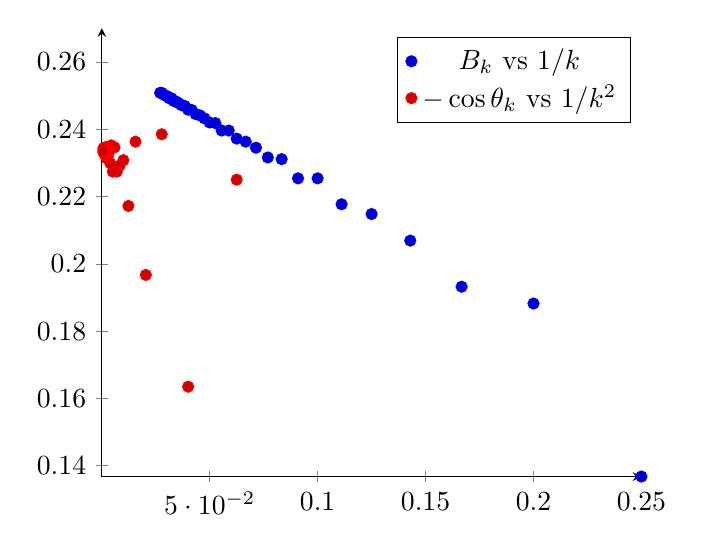
\begin{tikzpicture}
\begin{axis}[axis x line=middle, axis y line=middle
,xmin=0,ymax=0.27]
\addplot +[only marks,mark=*] coordinates {

(0.25,0.1368)

(0.2,0.1882)

(0.1667,0.1932)

(0.1429,0.2069)

(0.125,0.2148)

(0.1111,0.2177)

(0.1,0.2254)

(0.09091,0.2254)

(0.08333,0.2311)

(0.07692,0.2316)

(0.07143,0.2345)

(0.06667,0.2363)

(0.0625,0.2372)

(0.05882,0.2396)

(0.05556,0.2396)

(0.05263,0.2418)

(0.05,0.242)

(0.04762,0.2432)

(0.04545,0.2441)

(0.04348,0.2445)

(0.04167,0.2457)

(0.04,0.2458)

(0.03846,0.2469)

(0.03704,0.2471)

(0.03571,0.2477)

(0.03448,0.2482)

(0.03333,0.2484)

(0.03226,0.2492)

(0.03125,0.2492)

(0.0303,0.2498)

(0.02941,0.25)

(0.02857,0.2503)

(0.02778,0.2508)

(0.02703,0.2508)

};
\addlegendentry{\(B_k\) vs \(1/k\)};


\addplot +[only marks,mark=*] coordinates {

(0.0625,0.225)

(0.04,0.1635)

(0.02778,0.2385)

(0.02041,0.1967)

(0.01563,0.2363)

(0.01235,0.2172)

(0.01,0.2308)

(0.008264,0.2292)

(0.006944,0.2274)

(0.005917,0.2346)

(0.005102,0.2274)

(0.004444,0.2352)

(0.003906,0.2299)

(0.00346,0.2335)

(0.003086,0.2329)

(0.00277,0.2318)

(0.0025,0.2346)

(0.002268,0.2314)

(0.002066,0.2347)

(0.00189,0.2323)

(0.001736,0.2337)

(0.0016,0.2337)

(0.001479,0.2328)

(0.001372,0.2345)

(0.001276,0.2326)

(0.001189,0.2344)

(0.001111,0.2332)

(0.001041,0.2338)

(0.0009766,0.2339)

(0.0009183,0.2332)

(0.0008651,0.2344)

(0.0008163,0.2331)

(0.0007716,0.2342)

(0.0007305,0.2335)


};
\addlegendentry{\(-\cos\theta_k\) vs \(1/k^2\)};
\end{axis}
\end{tikzpicture}

&
\parbox[b]{0.3\linewidth}{\caption{\label{fig:tiwdbcDS}%
generalised Domb--Sykes plot (Mercer \& Roberts, 1990) to show convergence for \(|\gamma|<3.8\) due to a convergence limiting singularity at angle~\(103^\circ\) to the real \(\gamma\)-axis.}}
\end{tabular}
\end{figure}
}{}





Fin.
\begin{reduce}
end;
\end{reduce}


\end{document}
